\section{Linear Optical Quantum Computing}
Trapped Ion Quantum Computing looks like a very promising route for quantum computation but because the concepts qubits and entanglement aren't limited to any one particular implementation but revolve around a quantum system (or systems) there exists multiple ways thought of (and achieved) to create these new types of computers, the method we'll look at in this section uses photons to represent qubits and then performs operations on those photons which represents quantum logic gate operations on qubits. Linear Optical Quantum Computing is the name used for photonic quantum computers that make use of classical linear optical tools such as beamsplitters, polarisers, phase shifters, etc. to perform these operations but the most interesting thing (at least in our opinion) when it comes to building LOQC's is the protocol which is used that makes a photonic quantum computer viable at the large qubit scale (this protocol makes use of quantum teleportation and we'll cover both at the end of this section). Before we discuss this, however, we need to talk about how we make photons into qubits. 

\subsection{Types of Encoding}
When we talk about the ways in which a photon can be made to represent a qubit we are talking about the method of "encoding". Much like the different methods for quantum computing in general, there are many different ways we can encode photons to represent qubit states; there exists mixed polarisation encoding, parity encoding etc. but for the purposes of this article we'll focus on spatial encoding, specifically "dual rail" encoding. 

\subsubsection{Spatial Modes}
Single Rail encoding involves sending a photon down a single rail or cavity, imagine a photon travelling down a wire. We then say the existence of a photon in the rail is representative of a qubit with state $\ket{1}$ and then nothing but vacuum in the rail is representative of a qubit in state $\ket{0}$. Dual rail encoding is very similar but instead of a single rail/cavity there are two. In this case we can label the rails (sometimes called modes) A and B; when a photon is detected in mode A but not B this is representative of a qubit with the state $\ket{0}$ abd when a photon is detected in mode B but not A this is representative of a quibt with the state $\ket{1}$. \\ So what is the difference between these types of encoding? As it turns out, performing 2 qubit gate operations (and then entangling multiple qubits) in a single rail encoded quantum computer is very simple, it involves the use of a linear optical tool called the beamsplitter and the phenomena known as the Hong-Ou-Mandel effect (both of these we discuss in more detail later) but in a dual-rail representation achieving this deterministically isn't physically possible. Similarly, in the dual rail representation, performing 1 qubit operations is quite simple but is not physically possible to achieve deterministically in the single rail representation. For the rest of this section we will have a heavy focus on the dual-rail representation and we'll discuss how non-deterministic, or rather probabilistic, tools are used to create 2 qubit gate operations here. We should note that mathematically the horizontal-vertical polarisation representation is identical to the dual rail representation. 


%%%%%%%%%%%%%%%%%%%%%%%%%%%%%%%%%%%%%%%%%%

\subsection{Useful Linear Optical Tools and Single Qubit Representations}
Before we go into any of the complex techniques that really make photonic quantum computers seem like a viable, scalable direction for quantum computers of the future we need to discuss some of the basic tools that we can use to manipulate our photons and by extension, our qubits.
\subsubsection{Beam Splitters}
\begin{itemize}
    \item The name is very apt, beam splitters divide a beam of light into two beams with the intensity of each beam being dependent on the angle the beam splitter is placed at in relation to the incoming beam
    \item Depending on the type of encoding you choose, the 'beamsplitter' can be made in different ways due to the way it effects the photon but in our dual rail encoding the beamsplitter is made of two glass prisms placed back to back with a half-silvered mirror placed in between them %place image of this from QC&QI
    \item When we apply a beamsplitter to a qubit it is the equivalent of performing some form of transformation to the state of that qubit, this transformation can be represented as $B_{\theta\phi} = $ $\begin{pmatrix}
    cos(\theta) & -e^{i\phi}sin(\theta) \\
    e^{-i\phi}sin(\theta) & cos(\theta) 
    \end{pmatrix}$ where $\theta$ is related to the transmission and reflection amplitudes of the outgoing beams (the reflection amplitude R= $sin^2(\theta)$ and the transmission amplitude T = 1-R = $cos^2(\theta)$) and $\phi$ is the phase shift applied by the beamsplitter
    \item It should be noted that the Pauli X gate can be constructed from this beamsplitter by setting $\theta = \phi = \frac{\pi}{2}$
    
\end{itemize}
\subsubsection{Phase Shifters}
\begin{itemize}
    \item Phase shifters are an even simpler tool but very useful. 
    \item We simply use a material that has a higher refractive index than air (or whichever medium our photons are travelling through in the rails) and have the beams pass through this medium to phase shift them
    \item The phase shifter performs a transformation on the qubit that can be described as $P_\phi = $ $\begin{pmatrix}
    1 & 0 \\
    0 & e^{i\phi}
    \end{pmatrix}$ where the phase shift $\phi$ is given by the thickness and refractive index of the phase shifter.
    \item An important thing to note that applies for all phase shift gates (and not just specifically the optical one we describe here) is that when $\phi = \frac{\pi}{2}$ then this phase shift gate is equivalent to the Pauli Z transformation.
\end{itemize}
\subsubsection{Mirror}
\begin{itemize}
    \item A mirror is even simpler than the tools listed before. As you likely already know, a mirror simply reflects our beams with near 100\% intensity.
    \item We can describe the action of a mirror on our photonic qubit as a special case of the beamsplitter where the reflection intensity is 100\% and the phase shift $\phi = 0$
\end{itemize}
\subsubsection{Photodetectors}
\begin{itemize}
    \item A photodetector detects the arrival of photons. It accomplishes this by converting the energy deposited by the photon onto its surface into an electrical signal which can be measured and quantified.
    
    \item The quantum efficiency $\eta$ of a photodetector is the probability that a single incident photon generates an electrical signal that contributes to the overall detector current.
    
    \item This component is crucial in an optical quantum computer as it allows the readout of the output of the quantum computer.
\end{itemize}
\subsubsection{Kerr Media}

\begin{itemize}
    \item The most important property of a Kerr medium is the cross-phase modulation it provides.  
    \item For a two qubit register, Kerr media has the following effect:
    
    \begin{align*} 
    K \ket{00} &=  \ket{00}\\
    K \ket{01} &=  \ket{01}\\
    K \ket{10} &=  \ket{10}\\
    K \ket{11} &=  e^{i\chi L}\ket{11}
    \end{align*}
    
    \item If the cross-phase modulation $\chi L$ is taken to be $\pi$, then $K \ket{11} &=  -\ket{11}$. This can be expressed as a matrix K acting on two qubits. 
    
    $$K = \begin{pmatrix}
    1 & 0 & 0 & 0\\
    0 & 1 & 0 & 0\\
    0 & 0 & 1 & 0\\
    0 & 0 & 0 & -1\\
    \end{pmatrix}$$
    
    \item If the matrix K were then left and right multiplied by the Hadamard gate acting individually on both qubits, a C-NOT gate can be constructed.
    
    \item If this were the only method to entangle photons, a single photon quantum computer would be extremely hard to physically construct. The needed nonlinear Kerr media with large ratio of cross phase modulation to absorption loss are difficult to create. It is theoretically estimated that, in the best possible case, approximately 50 photons must be absorbed for each photon which experiences a $\pi$ phase modulation.
\end{itemize}


%%%%%%%%%%%%%%%%%%%%%%%%%%%%%%%%%%%%%%%%%%



%%%%%%%%%%%%%%%%%%%%%%%%%%%%%%%%%%%%%%%%%%%

\subsection{Two Qubit Operations}
With our dual rail encoding of a linear quantum computer it turns out that implementing a two qubit operation is quite difficult. Physically this is fairly easy to understand, manipulating photons to interact with each other is quite difficult but what is interesting is that this problem persists no matter the type of encoding we use; for single rail encoding implementing two qubit operations is fairly easy but single qubit operations becomes difficult. The Bougoliubov transformation which describes the linear optical circuit that is supposed to transform our computational basis states into the maximally entangled Bell states is described by .... \\ Given that these are different we cannot actually reach maximal entanglement in a deterministic way (maximal entanglement can be achieved with the most simple of two qubit gates and so this implies that two qubit gates cannot be implemented deterministically either). To work around this we could implement the use of Kerr media as discussed above but for the purpose of keeping this guide readable, we'll focus on the far more interesting probabilistic methods.


\subsubsection{Control-Z gate (Control Phase Shift Gate)}
We start by talking about the Hong-Ou-Mandel (HOM) effect. This is an interesting phenomenon that plays a pivotal role in optical quantum computing. Imagine two photons enter a 50:50 beamsplitter from rails A and B which can be written as $\ket{1,1}_{a,b}$. This state can be written in terms of the creation operators $\hat{a}^\dagger$ (acting on A) and $\hat{b}^\dagger$ (acting on B) in the following way $\hat{a}^\dagger\hat{b}^\dagger\ket{0,0}$. When the photons exit the beamsplitter there is a 50:50 chance that the photons could come out through rail C or rail D and so by going through the beamsplitter the state $\hat{a}^\dagger\hat{b}^\dagger\ket{0,0}_{a,b}$ is transformed into $\frac{1}{2}((\hat{c}^\dagger)^2 - (\hat{d}^\dagger)^2)\ket{0,0}_{c,d}$ \footnote{ the beamsplitter transforms $\hat{a}^\dagger\ket{0}_a$ into the state $\frac{1}{\sqrt{2}}(\hat{c}^\dagger + \hat{d}^\dagger)\ket{0}_c$ whilst transforming  $\hat{b}^\dagger\ket{0}_b$ into the state $\frac{1}{\sqrt{2}}(\hat{c}^\dagger - \hat{d}^\dagger)\ket{0}_c$. Physically this can be described as the photon from rail B being phase shifted by $\pi$ when reflected from the beamsplitter and going into rail D}. This is important because if we remember that $\hat{a}^\dagger, \hat{b}^\dagger, \hat{c}^\dagger$ and $\hat{d}^\dagger$ are creation operators then this is equivalent to $\frac{1}{\sqrt{2}}(\ket{2,0}_{c,d} - \ket{0,2}_{c,d})$. In words, when 2 photons coming from different rails enter into a 50:50 beamsplitter at the same time, they will both go down the exact same rail together, either C or D, but they will not exit in different rails like they came. This can be described as photon bunching but it is known as the Hong-Ou-Mandel effect and "lies at the heart of linear optical quantum computing" (cite peter kiok). \\
As stated earlier, implementing two-qubit gates must have some probabilistic, non deterministic element to them and to achieve this we will be using the non deterministic sign shift gates which we'll cover in more detail in the next section but the important thing to note now is that when looking at the 3 lowest Fock states, these NS gates phase flip the 3rd lowest:
\begin{equation} \label{NS evolution}
    \alpha\ket{0} + \beta\ket{1} + \gamma\ket{2} \rightarrow \alpha\ket{0} + \beta\ket{1} - \gamma\ket{2}
\end{equation}

\begin{figure}[h]
    \centering
    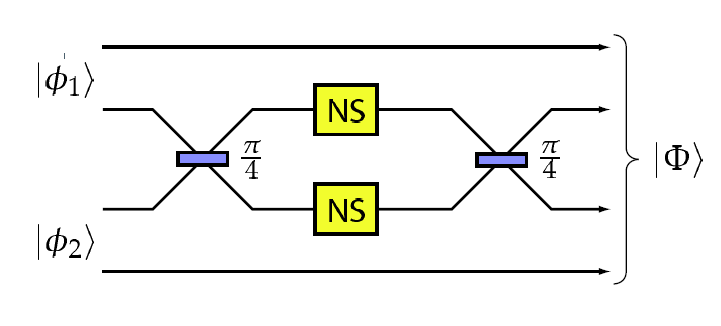
\includegraphics[width=0.9\textwidth]{images/CZ-gate.png}
    \caption{Circuit for probabilistic CZ gates in LOQC using NS gates}\label{fig:CZ_gate}
\end{figure}

As we can see in \ref{fig:CZ_gate}, when $\ket{\phi_1}$ and $\ket{\phi_2}$ are both equal to $\ket{1}$ then there will be a photon in the middle two modes ($\ket{\phi_2}$ is flipped). This means that the two photons will interact at the first beamsplitter, via the Hong-Ou-Mandel effect they will "bunch" and go down the same mode together towards the NS gate. The NS gate will sign shift the photons in the mode they went down due to the NS evolution \ref{NS evolution} and then the photons will interact with the second beamsplitter to finally give the state $-\ket{1,1}$.%\textbf{EVERYTHING AFTER THIS IS WRONG} What makes this circuit interesting is that because of the HOM effect, this situation only occurs when $\ket{\phi_1}$ and $\ket{\phi_2}$ are both equal to $\ket{1}$. In the case where only one photon goes through the middle modes, the photon will be split by the beam splitter into both modes, each mode will interact with the NS gate, acquiring a phase shift each but these phase shifts destructively cancel when the modes are brought together at the second beam splitter and the HOM effect occurs again. Due to the fact that the NS gate has a 1/4th probability of operating correctly and this gate requires two in tandem, the probability of the CZ gate operating as we expect is $p_{CZ} = p_{NS}^2 $

\subsubsection{Nonlinear sign shift gate}
As stated above, the nonlinear sign shift gate is a very useful tool as its non-deterministic effects allow us to achieve maximally entangled states when we otherwise couldn't but how is the NS gate made? The circuit is actually fairly simple; it involves 2 ancillary modes, one with a photon present and the other without, 3 beam splitters set at differing angles with no phase shift and then 2 "perfect" photon detectors. We can see this in \ref{fig:NS_gate}. Going through each case for this NS gate is quite exhaustive which we won't cover here but the important thing to note is that 1/4 of the time the fock states $\alpha\ket{0}$ and $\beta\ket{1}$ are left untouched and when two photons come through from $\phi$, $\gamma\ket{2} \rightarrow -\gamma\ket{2}$ 

\begin{figure}[h]
    \centering
    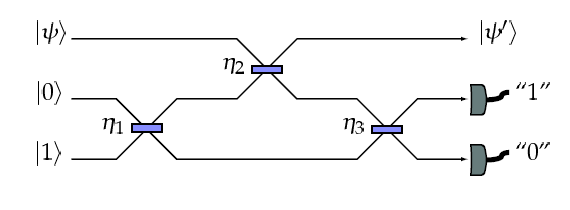
\includegraphics[width=0.9\textwidth]{images/NS gate.png}
    \caption{Circuit for probabilistic NS gates in LOQC using ancillary modes}\label{fig:NS_gate}
\end{figure}
%%%%%%%%%%%%%%%%%%%%%%%%%%%%%%%%%%%%%%%%%%



\subsection{Efficiency}
As we know by now, the real magic of quantum computation occurs when we can implement two qubit gates as this allows us to perform quantum entanglement between qubit states which is then instrumental in many other constructs such as Quantum Teleportation, Quantum Algorithms, etc.

The issue we tend to run across with LOQC is that photons tend to not naturally interact with each other. This makes the practical implementation of a two qubit gate a very difficult task. One suggested method is to use nonlinear Kerr media to provide a cross phase modulation of $\pi$ between photon states. This combined with a beamsplitter can be used to construct a CNOT gate, from which a universal set of gates can be obtained. However, as stated in Section 7.4.3 in \cite{nielsen_chuang_2010}, obtaining nonlinear Kerr media with the sufficient cross phase modulation is not possible without incurring an excessive absorption loss: for every photon that incurs a $\pi$ cross phase modulation, approximately 50 photons must be absorbed. Another suggested method of overcoming this uses photo-detectors to make projective measurements which can induce an interaction between photons\cite{Kok:2005jip}. This is a probabilistic approach with the probability of success being rather small and the method for increasing this probability to "near-one" values scales exponentially with resources (optical modes required). This makes optical computation seem quite unfeasible on the large scale but thanks to a few interesting results in quantum optics we can implement what is referred to as the KLM protocol to construct scalable 2-qubit gates.


\subsubsection{Three results that allow for efficient LOQC}
Due to the following results the additional resources for a LOQC that scales with n, scales with O($n^2$):
\begin{itemize}
    \item Non-deterministic quantum computation is possible with linear optics
    \item The probability of success can be increased close to one
    \item The resources needed for "accurately" (probability of success close to 1) encoded qubits scales efficiently  
\end{itemize}

\subsection{Scalability and the KLM Protocol}
As you probably might have guessed by now, there is a major problem with photonic quantum computing as we've discussed that uses probabilistic gates and that is the fact that the probabilities of these gates are quite low. Having a CZ gate that only works 1/nth of the time means that to get some reasonable result we need to run our circuit n times. As we implement more complicated circuits that involve some number, n, of deterministic gates with probabilities $\frac{1}{p}$, the chance of success of our circuit is $\frac{1}{p^n}$. This is obviously infeasible as any interesting circuit will require many gates and with our current set-up that means any scalable photonic quantum computer is too resource intensive to be worth it. \par
This alone sounds like it would be the nail in the coffin for further development into LOQC's but using quantum teleportation, the discrete quantum Fourier transform and n number of photonic modes the probability of success for a given non-deterministic gate can become 'near-deterministic' with a success rate of $\frac{n^2}{(n+1)^2}$ which tends to 1 as n becomes sufficiently large. This is a process named the KLM protocol after Knill, Leflamme and Milburn after it was developed in 2000 and it is essential for any photonic quantum computer we could hope to build on a scale larger than a few gates.

\subsubsection{How does Quantum Teleportation work?}

\begin{itemize}
    \item quantum teleportation is not as luxurious as it sounds, we're simply transferring the state of one qubit to another exactly but the state of the original qubit is destroyed which we can imagine is a result of the no-cloning theorem. The best part about this is that we do not need any information about the original state which means that in quantum teleportation, the original state doesn't deconstruct as we 'teleport' it to another qubit
    \item The process is as followed:
    \begin{itemize}
        \item Eve prepares 2 entangled qubit and passes one to Alice and one to Bob without them deconstructing. 
        \item Alice has 2 qubits, the one Eve gave and the one she wants to teleport. She then proceeds to perform a Bell Measurement on the 2 qubits she has which gives one of 4 possible outcomes \textit{no matter the state of her original qubit}. 
        \item She then classically tells Bob which of the 4 outcomes she got.
        \item Bob then uses this information to perform one of 4 possible procedures to his qubit (the one prepared by Eve) and upon performing this procedure his qubit will be in the exact state Alice's qubit was before the Bell Measurement.
    \end{itemize}
    
\end{itemize}

\begin{itemize}
    \item How teleportation works
    \item How the commutativity of the cz gate and the x and z gates means that we can prepare the cz gate 'offline' (we can prepare these ahead of time using several trials and then store it for use later) with the entangled qubits that make teleportation work - the qubits we want to apply the cz gate on can then be teleported onto modes that have had the cz gate applied to them.
    \item If teleportation was deterministic then the probabilistic part (the cz gate) will have been moved offline, meaning that with enough preparation (and storage) our qc's would never fail but the bell measurements that make teleportation work are only successful half the time, given that there are two bell measurements being made, this modified cz-gate is back to the same probability
    \item KLM Near deterministic teleporter
\end{itemize}
\subsection{Fault tolerance}
\subsubsection{Photon loss}